\section{实验}
\subsection{协议}
模型为Meta-Llama-3.1-8B-Instruct。Vector-GSQ锚点使用FineWeb-Edu 4096 train/128 validation/512 Vector-GPTQ，序列长度4096。任务适应只开放layers 28--31；ARC-C、ARC-E、HellaSwag、PIQA与WinoGrande各使用512 train、256 validation及固定offset 1088后的31条audit。文本使用4096/128/64条train/validation/audit，长度4096；新cache前5440行与旧缓存bit-exact。训练2 epochs，固定seed0，不扫描LR、group、projection ratio或seed。PPL使用WikiText2 test、seqlength 2048；准确率使用全量0-shot ARC-C、ARC-E、HellaSwag、LAMBADA、PIQA和WinoGrande。正式实验只使用一张A100 80GB。

\subsection{安全交接与正式端点}
\begin{figure*}[t]
\centering
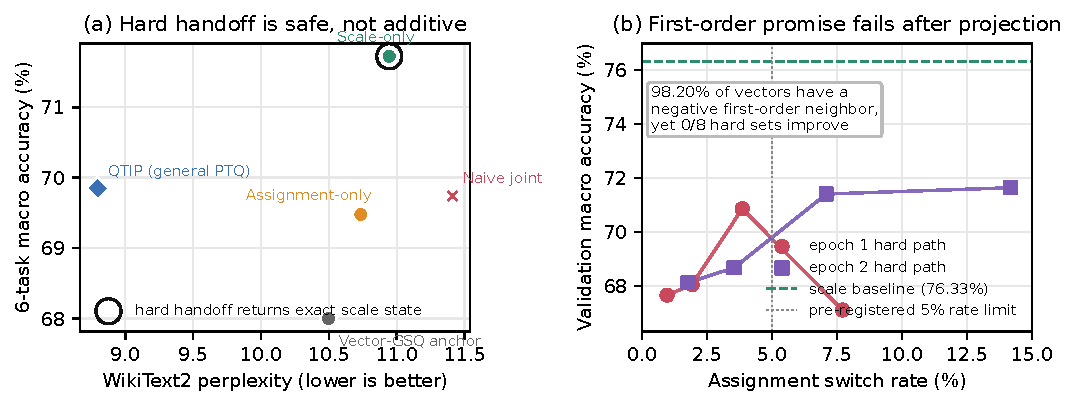
\includegraphics[width=0.95\textwidth]{../img/v10_hard_handoff.pdf}
\caption{左：hard handoff精确返回scale-only，说明部署态被保护但无组合增益。右：八个真实hard projection均低于scale baseline，尽管$98.20\%$向量具有负一阶邻居。}
\label{fig:v10}
\end{figure*}

\begin{table}[t]
\centering
\small
\caption{同模型完整部署端点。QTIP未使用任务标签，只作通用PTQ坐标。}
\begin{tabular}{lccc}
\toprule
端点 & PPL$\downarrow$ & Macro-6$\uparrow$ & 五任务$\uparrow$\\
\midrule
QTIP & \textbf{8.7971} & 69.8469 & 69.8749\\
Vector-GSQ锚点 & 10.4960 & 67.9997 & 68.1046\\
Assignment-only & 10.7347 & 69.4774 & 69.0744\\
Scale-only & 10.9448 & \textbf{71.7223} & \textbf{72.5484}\\
Naive joint & 11.4098 & 69.7434 & 68.9511\\
Hard handoff & 10.9448 & \textbf{71.7223} & \textbf{72.5484}\\
\bottomrule
\end{tabular}
\end{table}

Naive joint被scale-only严格支配，说明soft共享状态产生破坏；hard handoff与scale-only重合，说明状态一致后当前assignment proposal仍无增量硬解。Assignment-only仍比锚点提高1.48 pp且PPL漂移更小，因此它是独立Pareto分支，而非在scale后可叠加模块。

\subsection{一阶负方向与八个硬集合}
Scale baseline validation Macro为$76.3281\%$，balanced loss为0.679691。$145{,}465{,}344$个向量的加权负一阶率为$98.1965\%$，各Linear为$97.4782\%$--$98.3283\%$。
\begin{table}[t]
\centering
\small
\caption{Scale硬锚点后的所有嵌套部署投影。}
\begin{tabular}{cccccc}
\toprule
Epoch & 投影 & 切换率 & Macro$\uparrow$ & Loss$\downarrow$ & Gate\\
\midrule
-- & source & 0 & \textbf{76.328} & \textbf{0.680} & --\\
1 & 1/8 & 0.964 & 67.656 & 0.866 & fail\\
1 & 1/4 & 1.927 & 68.047 & 0.836 & fail\\
1 & 1/2 & 3.854 & 70.859 & 0.790 & fail\\
1 & full & 7.708 & 67.109 & 0.910 & fail\\
2 & 1/8 & 1.771 & 68.125 & 0.841 & fail\\
2 & 1/4 & 3.542 & 68.672 & 0.830 & fail\\
2 & 1/2 & 7.083 & 71.406 & 0.778 & fail\\
2 & full & 14.167 & 71.641 & 0.736 & fail\\
\bottomrule
\end{tabular}
\end{table}
在预注册$5\%$ rate内，最佳changed点仍低5.47 pp、loss高$16.24\%$；放宽后最佳changed endpoint也低4.69 pp、loss高$8.32\%$。失败不能归因于full过密或只差一个projection ratio。

\subsection{Audit、合同与成本}
所有changed候选在validation已失败，因此没有非零状态进入audit；summary中的audit flag为false表示audit未被调用接受changed candidate，并非非零候选audit失败。最终epoch0/no-op的assignment、scale、codebook、normalizer、固定元数据和非目标状态均精确不变，fresh reconstruction误差为0。正式六任务分别为53.7543、78.5774、77.5443、67.5917、79.5430和73.3228，Macro-6为$71.7223\%$；PPL 10.9447565，逻辑码率2.1207557 bpp。

Calibration及八个hard projection用时6.65 h、峰值31.80 GiB；PPL用时55.48 s，六任务评测26.45 min。首轮4.93 h诊断run暴露旧selector只有full先通过才评估sparse的逻辑错误；修复后每个投影独立Gate，失败run与测试均保留。

\subsection{边界与下一假设}
QTIP在无任务标签设置具有更低PPL和名义码率；本文不能以task-scale宣称同监督SOTA。PV-Tuning已覆盖一般坐标交替，当前结果也没有给出相对其正优势。现象只在该模型、最后四层、8-way候选和当前监督上成立，不能推出scale普遍耗尽assignment自由度，也未证明曲率是唯一根因。下一实验应以scale-conditioned曲率惩罚或跨batch/任务梯度一致性筛选alternative；若仍no-op，应停止把assignment作为scale后续主模块。
